\documentclass[]{politex}
% ========== Opções ==========
% pnumromarab - Numeração de páginas usando algarismos romanos na parte pré-textual e arábicos na parte textual
% abnttoc - Forçar paginação no sumário conforme ABNT (inclui "p." na frente das páginas)
% normalnum - Numeração contínua de figuras e tabelas 
%	(caso contrário, a numeração é reiniciada a cada capítulo)
% draftprint - Ajusta as margens para impressão de rascunhos
%	(reduz a margem interna)
% twosideprint - Ajusta as margens para impressão frente e verso
% capsec - Forçar letras maiúsculas no título das seções
% espacosimples - Documento usando espaçamento simples
% espacoduplo - Documento usando espaçamento duplo
%	(o padrão é usar espaçamento 1.5)
% times - Tenta usar a fonte Times New Roman para o corpo do texto
% noindentfirst - Não indenta o primeiro parágrafo dos capítulos/seções


% ========== Packages ==========
\usepackage[utf8]{inputenc}
\usepackage{amsmath,amsthm,amsfonts,amssymb}
\usepackage{graphicx,cite,enumerate}
\usepackage{float}


% ========== Language options ==========
\usepackage[brazil]{babel}
%\usepackage[english]{babel}


% ========== ABNT (requer ABNTeX 2) ==========
%	http://www.ctan.org/tex-archive/macros/latex/contrib/abntex2
%\usepackage[num]{abntex2cite}

% Forçar o abntex2 a usar [ ] nas referências ao invés de ( )
%\citebrackets{[}{]}


% ========== Lorem ipsum ==========
\usepackage{blindtext}



% ========== Opções do documento ==========
% Título
\titulo{Sistema Web para Instalação de ERBs}

% Autor
\autor{Eric Rodrigues Pires \\%
       Mateus Nakajo de Mendonça}

% Para múltiplos autores (TCC)
%\autor{Nome Sobrenome\\%
%		Nome Sobrenome\\%
%		Nome Sobrenome}

% Orientador / Coorientador
\orientador{Bruno de Carvalho Albertini}
%\coorientador{Nome do coorientador (opcional)}

% Tipo de documento
\tcc{de Computação}
%\teseDOC{Engenharia Elétrica}
%\teseLD
%\memorialLD

% Departamento e área de concentração
\departamento{PCS}
%\areaConcentracao{Área de concentração}

% Local
\local{São Paulo}

% Ano
\data{2018}




\begin{document}
% ========== Capa e folhas de rosto ==========
\capa
\falsafolhaderosto
\folhaderosto


% ========== Folha de assinaturas (opcional) ==========
%\begin{folhadeaprovacao}
%	\assinatura{Prof.\ X}
%	\assinatura{Prof.\ Y}
%	\assinatura{Prof.\ Z}
%\end{folhadeaprovacao}


% ========== Ficha catalográfica ==========
% Fazer solicitação no site:
%	http://www.poli.usp.br/en/bibliotecas/servicos/catalogacao-na-publicacao.html


% ========== Dedicatória (opcional) ==========
\dedicatoria{Dedicatória}


% ========== Agradecimentos ==========
\begin{agradecimentos}

Thanks...

\end{agradecimentos}


% ========== Epígrafe (opcional) ==========
\epigrafe{%
    \emph{``Epígrafe''}
    \begin{flushright}
        -{}- Autor
    \end{flushright}
}


% ========== Resumo ==========
\begin{resumo}
Este projeto de formatura tem como objetivo criar um sistema capaz de calcular
posições para a instalação de Estações Radiobase (ERBs) de forma que a
cobertura da rede de ERBs seja máxima. A partir da região dada como entrada, o
sistema obterá seus dados geográficos através de um Sistema de Informações 
Geográficas (SIG) e utilizará programação específica para a otimização da posição
de instalação. Para interface com o usuário do sistema, criaremos uma aplicação
Web responsiva que permita selecionar a região na qual se pretende instalar uma
ERB e mostra as posições ideais para instalação.
\\[3\baselineskip]
%
\textbf{Palavras-Chave} -- Estações~Radiobase, Otimização, Sistema~de~
Informações~Geográficas, Aplicação~Web.
\end{resumo}


% ========== Abstract ==========
\begin{abstract}
This term paper intends to achieve a system capable of calculating the position
to install cellular Base Stations (BS) so that we maximize the coverage network.
From a given input region, the system will collect geographic data through a
Geographical Information System (GIS) and utilize specific programming to optimize
the placement position. For interfacing with the system user, we will develop a
responsive Web application that allows the selection of a region on which we
intended to place a BS, and show the ideal points for installation.
\\[3\baselineskip]
%
\textbf{Keywords} -- Base~Stations, Optimization, Geographical~Information~
System, Web~Application.
\end{abstract}


% ========== Listas (opcional) ==========
\listadefiguras
\listadetabelas

% ========== Listas definidas pelo usuário (opcional) ==========
\begin{pretextualsection}{Lista de símbolos}

\textbf{ERB:} Estação Radiobase

\textbf{SIG:} Sistema de Informações Geográficas

\textbf{TCC:} Trabalho de Conclusão de Curso

\end{pretextualsection}

% ========== Sumário ==========
\sumario



% ========== Elementos textuais ==========

\chapter{Introdução}
Na revolução da informação em que vivemos hoje, em que cada vez mais pessoas
estão conectadas à rede, o acesso à Internet tem se tornado cada vez mais
essencial no dia-a-dia, até mesmo a populações consideradas isoladas. Empresas
bem conhecidas, como Vivo e Claro, vêm se empenhando para garantir melhor
acesso a mais pessoas, mas se deparam com problemas de engenharia nesta
tarefa.

A extensão territorial e a densidade demográfica desigual do Brasil são dois
dentre vários fatores que tornam problemas de telecomunicação mais complexos.
A dimensão deste problema gera um grande potencial de mercado para empresas
terceirizadas, voltadas à instalação de Estações Radiobase (ERBs) para
compartilhamento ou aluguel de células telefônicas às grandes empresas de
telecomunicação. Dessa forma, há demanda do mercado por ferramentas que
simplifiquem e/ou automatizem a tarefa de estudo de localização de ERBs.

\section{Objetivo}
O objetivo deste projeto de formatura é criar um sistema que permita calcular
posições para a instalação de antenas de telefonia de forma a maximizar o
alcance delas. Com esse fim, levaremos em conta dados geográficos para
realizarmos os cálculos.

Também é de grande importância que tal sistema tenha uma interface prática
para os usuários. Portanto, uma interface web que apresente os dados
requisitados é essencial para o projeto.

Outras possíveis ramificações do projeto para showcase ao público geral, que não
é o público-alvo, é a localização de antenas a partir do próprio celular do
usuário, e a estimativa de posição do dispositivo pelas antenas encontradas.

\subsection{Sistema de Informação Geográfica}
Um SIG (Sistema de Informação Geográfica) é um sistema computacional capaz de
obter, gravar, gerir, analisar e visualizar dados geográficos. Seu uso permite
tomar decisões, analisar estatísticas e resolver problemas de otimização a
partir de dados geográficos. O SIG pode ser usado tanto em lojas de varejo para
decidir onde abrir uma nova filial, como em rastrear padrões de migração,
controle e o monitoramento do desmatamento, planejamento urbano, etc.

No nosso projeto, usaremos um software SIG para gravar e exibir a posição de
ERBs (Estações Radiobase) atuais, o relevo e os consumidores atingidos pela
rede de ERBs. Com essas informações, determinaremos as posições ótimas de
ERBs de modo a maximizar a área de cobertura do sistema de telefonia.
Para tanto, aplicaremos técnicas de programação linear, uma vez que
estamos diante de um problema de otimização cuja função a ser otimizada
é linear em relação às variáveis de entrada.

\subsection{Interface Web}
Para interação com o usuário, criaremos um front-end de uma aplicação Web que
permita selecionar a região na qual se pretende instalar alguma ERB.
Esta interface se comunicará com o back-end do SIG, para obter e calcular os
dados desejados.

O design deverá ser responsivo, podendo ser utilizado em plataformas mobile
ou desktop, e simples, com opções simples para apenas verificar a posição ótima
de instalação de antenas em determinada área escolhida pelo usuário. Para isso,
a interface deverá exibir um mapa, como por exemplo o da plataforma
OpenStreetMap, com as informações do SIG, que permita ao usuário selecionar uma
área desejada. Os dados serão calculados no back-end e exibidos ao usuário na
tela. Para isso, será necessário desenvolver um front-end possivelmente
dinâmico.

\section{Motivação}
Com uma análise preliminar do setor, verificamos o mercado de instalação e
aluguel de torres telefônicas no Brasil para comparar as tecnologias utilizadas
em softwares ou pesquisas de  de ERBs. Há várias técnicas empregadas, desde
programação não-linear a algoritmos evolutivos, algoritmos de polinização a
programação inteira mista. Será feita uma comparação das tecnologias para
verificar a que mais se adequa ao nosso caso de uso.

Também pesquisamos serviços similares da concorrência. Um dos
produtos encontrados, chamado Atoll, é um software de planejamento de células e
posições de ERBs, similar ao que desejamos desenvolver, porém com 
funcionalidades estendidas como manutenção e melhoria de locais 
pré-estabelecidos, e parâmetros avançados de especificação das antenas, além de
módulos para outras tecnologias de telecomunicação como Wi-Fi \cite{atoll}.
Porém, a ferramenta parece muito voltada à instalação urbana e análise de
infra-estrutura pré-existente, sem foco em uma eventual expansão. Por isso,
vemos como que há necessidade do mercado por uma ferramenta voltada à ampliação
de uma rede de ERBs.

\section{Justificativa}
Sobre potenciais clientes, verificamos a existência de empresas no Brasil para
localizar antenas, alugar terrenos para a instalação de antenas ou alugar
antenas para empresas de telecomunicação. A maior parte destas empresas foca em
um contexto urbano, enquanto que há interesse das empresas de telecomunicação
e dos governos estaduais em expansão em áreas rurais.

MyTower é um portal de locação e venda de imóveis para operadoras de
telecomunicação \cite{mytower}. Ele permite que o usuário cadastre seu imóvel
e o anuncie para as operadoras após aprovação.
O portal então faz a intermediação entre o anunciante e a operadora.

A Skysites é uma empresa que oferece soluções na área da infraestrutura de
telecomunicação \cite{skysites}. Ela gere um portfólio de sítios para 
instalação de equipamentos de telecomunicação (torres, smallcells, rooftops,
etc), além de prover soluções customizadas para empresas de telecomunicação e 
compartilhar torres entre diferentes empresas. Outros serviços são redes para
cobertura \textit{indoor} e pequenas ERBs para melhorar a cobertura em ambiente
urbano, as \textit{small cells}.

\section{Organização do Trabalho}
No capítulo ``Introdução" deste trabalho, definimos a motivação da realização
deste sistema e o que buscamos alcançar neste projeto.

No capítulo ``Aspectos Conceituais'', será realizada a contextualização dos
conceitos empregados na área de aplicação e a revisão da literatura de base.

No capítulo ``Tecnologias Utilizadas'', listaremos as ferramentas, algoritmos
e dados necessários para o desenvolvimento do sistema deste trabalho.

No capítulo ``Metodologia do Trabalho'', definiremos os processos e fases
no desenvolvimento de funcionalidades deste sistema, como concepção, estudo,
projeto, implementação e testes.

No capítulo ``Especificação de Requisitos do Sistema'', definiremos os
requisitos do nosso sistema.


\chapter{Aspectos Conceituais}

\section{Algoritmos Avaliados}
Em consulta à literatura pré-existente sobre o problema de otimização de
instalação de ERBs, nos deparamos com várias abordagens distintas para o mesmo
problema, em diferentes níveis de abstração.

A princípio, nós nos voltamos a duas alternativas: LEE~et~al.~(2015)~
\cite{evolutivo} utiliza conceitos básicos de telecomunicações, através de uma
fórmula para calcular a satisfação dos usuários do sistema a partir de medidas
de qualidade de banda, se baseando em um algoritmo evolutivo para otimizar
a cobertura da rede. Já KARULKAR~\&~OH~(2016)~\cite{nao-linear} se baseia em
uma abordagem de limites geográficos impostos no processo de projeto de antenas,
utilizando programação não-linear para identificar a posição ótima.


\chapter{Tecnologias Utilizadas}

\section{Sistema Web}
No projeto, para facilidade de desenvolvimento, utilizaremos o framework Django,
escrito em Python. A integração de single-page com o back-end deverá ser feita
com o módulo de API REST do Django.

O Django possui funcionalidades de SIG pelo módulo GeoDjango, que utiliza como
banco de dados o PostGIS (baseado em Postgres). Serão armazenados
dados públicos de localização de ERBs, relevo e densidade populacional. Ele
será também responsável pelos cálculos realizados para a localização de novas
antenas.

Para interação com o usuário por um mapa interativo, utilizaremos a biblioteca
Leaflet, escrita em JavaScript. Ela se comunicará aos dados pela API REST a ser
desenvolvida, tanto para requisições quanto para exibições.

Optamos também pelo framework JavaScript conhecido por React, com a biblioteca
Redux, para realizar o controle \emph{single-page app} do nosso sistema, e a
interface gráfica Django Material para elaborar as telas do nosso sistema.

\section{Bases de Dados Utilizadas}
Utilizamos o Mapa de ERBs Brasil presente no portal Telebrasil \cite{mapa-erb}.
Essa base contém uma lista de ERBs do Brasil de novembro de 2017, com
informação de operadora, endereço, e posição geográfica de cada ERB.
Essas informações são essenciais para o cálculo da posição ótima da ERB para
maximizar a cobertura da célula.

Utilizamos também o OpenCelliD, da empresa Unwired Labs \cite{opencellid}.
Essa base contém uma lista de ERBs do mundo inteiro, com o CGI de cada ERB.
Os dados foram obtidos através da colaboração de usuários do aplicativo
LocationAPI da Unwired Labs. O LocationAPI trata-se de um serviço de
geolocalização que não depende de GPS. Dessa forma, com a base da OpenCelliD,
podemos estimar a posição de um celular a partir das ERBs as quais ele está
conectado.

Outra base de dados em estudo foi o Google Earth Engine \cite{earthengine}, uma
API específica para dados geográficos públicos do Google, como relevo e
densidade populacional. Devido à extensão destes dados, e à impraticidade de
armazenamento em banco próprio, será estudada a possibilidade de uma dependência
desta base através de sua API.

Mais duas bases de dados que serão utilizadas no projeto são: a G-Econ
\cite{gecon}, da Universidade de Yale, que apresenta os dados de paridade de
poder de comparar geograficamente; e o SIMET-NIC \cite{simet}, com o acesso e 
qualidade da Internet no Brasil. Acreditamos que estas duas bases de dados, em
conjunto com os anteriores, permitirão uma análise aprofundada de parâmetros
ótimos para a instalação de novas antenas.


\chapter{Metodologia do Trabalho}
Em uma primeira etapa, definimos com o orientador a proposta e o escopo deste
projeto, propondo a pesquisa a ser realizada tanto da perspectiva de
implementações quanto de requisitos necessários. Levantados tais requisitos no
capítulo ``Especificação de Requisitos do Sistema'', a próxima etapa se baseou
em projetar a realização de cada um destes requisitos de acordo com as
prioridades definidas, isto é, iniciar um processo de decisões definitivas para
o andamento do trabalho.

Feitas estas decisões, finalmente, realizou-se a prototipagem das nossas
funcionalidades, dividida entre os dois integrantes do grupo de forma paralela
para permitir o andamento de diferentes partes do sistema, com reuniões entre
os integrantes e o orientador para avaliar o progresso. Após esta análise
preliminar, iniciou-se o desenvolvimento definitivo do sistema na especificação
final, etapa que levará mais tempo neste projeto.

Por fim, antes de realizar a apresentação do trabalho final, será realizada uma
bateria de testes para verificar o funcionamento correto do sistema após o
desenvolvimento, sem a elaboração de novas funcionalidades, garantindo que
estamos dentro das nossas previsões de projeto.

Desta forma, nos organizamos para realizar a implementação do sistema, separando
as tarefas a serem realizadas nas categorias: pesquisa, projeto, e apresentação.
Utilizamos o cronograma oficial de TCC para elaborar um diagrama de Gantt na
Figura~\ref{fig:gantt} com a sequência de tarefas a serem divididas pelo grupo
ao longo do ano para cada semana. Indicamos também o período extra-escolar em
colunas azuis, aonde haverá desenvolvimento do sistema de forma mais lenta e
sem cronograma oficial.

\begin{figure}[H]
    \centering
    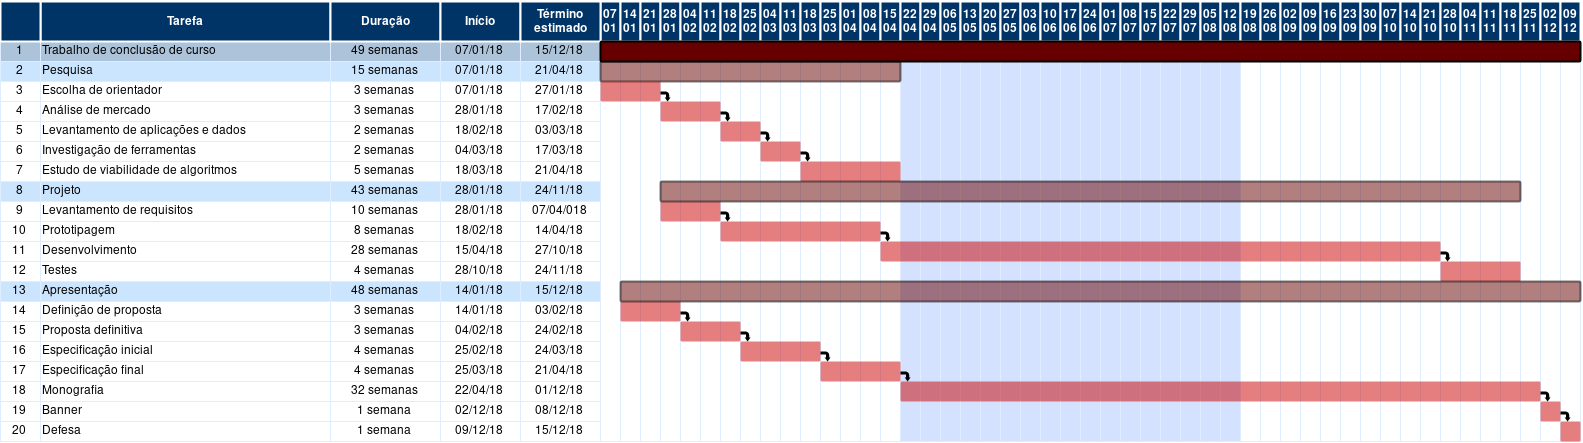
\includegraphics[width=6.5in]{imagens/diagrama_gantt}
    \caption{Diagrama de Gantt.}
    \label{fig:gantt}
  \end{figure}


\chapter{Especificação de Requisitos do Sistema}
Para definir os requisitos do nosso sistema, foi elaborada uma árvore de
pré-requisitos, listando a prioridade total dada a cada componente do sistema
final na Figura~\ref{fig:arvore_prerequisitos}.

\begin{figure}[H]
  \centering
  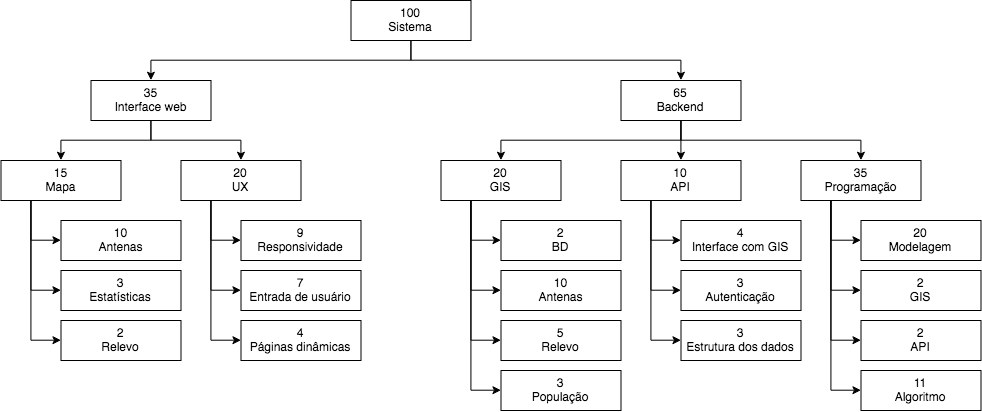
\includegraphics[width=6in]{imagens/arvore_prerequisitos}
  \caption{Árvore de pré-requisitos do sistema.}
  \label{fig:arvore_prerequisitos}
\end{figure}

Como evidenciado pela figura, a ênfase deste projeto será no back-end, em
especial na parte de modelagem e programação relacionadas ao cálculo de
otimização da posição de antenas. As outras duas partes relevantes do 
\emph{backend} tratam, respectivamente, do uso do banco de dados como SIG e da
comunicação externa de dados via API.

Embora tenha uma ênfase menor, o front-end da interface web também será
um requisito fundamental de projeto, separado na experiência do usuário e na
visualização do mapa.

Definido o escopo, começamos a pensar, junto ao nosso orientador, sobre os 
requisitos do projeto. A estratégia utilizada foi o brainstorming, leitura de 
obras de referência, e pesquisa de softwares com escopo parecido.
A ideia inicial era ter como ator principal do sistema o funcionário cadastrado
de uma empresa de instalação de antenas, porém depois consideramos que seria
complementar ao projeto considerar um usuário não-comercial, assim
como um usuário administrador. Nessa fase, perguntamo-nos como o nosso projeto
poderia ajudar esses atores, qual informação ele deveria produzir. Esse processo
nos levou à modelagem apresentada nas seções a seguir.

\section{Atores}
\begin{itemize}
\item Administrador
\item Funcionário cadastrado de Empresa de instalação de antenas
\item Usuário não-comercial
\end{itemize}

\section{Requisitos funcionais}
\begin{itemize}
\item Efetuar Login
\item Efetuar Logout
\item Cadastrar usuário no sistema
\item Exibir mapa com ERBs
\item Exibir mapa com cobertura celular estimada
\item Exibir localização ideal para instalação de uma nova ERB
\item Adicionar nova ERB
\item Fazer login por OAuth2
\item Acessar API
\item Exibir ERBs às quais o celular do usuário está conectado
\item Exibir mapa com qualidade do sinal por operadora
\item Estimar geolocalização do usuário
\item Listar usuários
\end{itemize}

\section{Requisitos não-funcionais}
\begin{itemize}
\item Funcionalidades e código bem documentados
\item Interface acessível e simples
\item Ser responsivo
\item Ser dinâmico
\item Ser rápido
\item Ser seguro   
\end{itemize}

\section{Descrição dos casos de uso}

\noindent \textbf{Caso de Uso 1}: Efetuar login no sistema. \\
\textbf{Descrição}: Este caso de uso descreve o processo de autenticação no sistema. \\
\textbf{Evento iniciador:} Usuário informa seu nome de usuário e senha. \\
\textbf{Atores:} Administrador, Funcionário ou Usuário não-comercial. \\
\textbf{Pré-condições:} Usuário entra na página de login. \\
\textbf{Sequência de Eventos:}
\begin{enumerate}
\item Usuário informa seu nome de usuário e sua senha.
\item Sistema autentica o usuário e senha.
\item Sistema exibe página inicial com opções correspondentes ao nível de privilégio do usuário.
\end{enumerate}
\textbf{Pós-condições:} Usuário logado no sistema. \\
\textbf{Extensões:} 
\begin{enumerate}
\item Usuário ou senha estão incorretos: sistema exibe mensagem de erro (passo 2).
\item Login por OAuth2: sistema recebe token de autenticação externa para o acesso (passo 1). 
\end{enumerate}
\textbf{Inclusões:} - \\

\noindent \textbf{Caso de Uso 2}: Efetuar logout no sistema. \\
\textbf{Descrição}: Este caso de uso descreve o processo de logout no sistema. \\
\textbf{Evento iniciador}: Usuário clica no botão de logout. \\
\textbf{Atores}: Administrador, Funcionário ou Usuário não-comercial. \\
\textbf{Pré-condições}: Usuário logado no sistema. \\
\textbf{Sequência de Eventos}: 
\begin{enumerate}
\item Usuário clica no botão de logout.
\item Sistema exibe página inicial para usuários não-logados.
\end{enumerate}
\textbf{Pós-condições}: Usuário não logado no sistema. \\
\textbf{Extensões}: - \\
\textbf{Inclusões}: - \\

\noindent \textbf{Caso de Uso 3}: Cadastrar usuário no sistema.  \\
\textbf{Descrição}: Este caso de uso descreve o cadastro de usuários no sistema \\
\textbf{Evento iniciador}: Usuário clica no botão cadastrar usuário. \\
\textbf{Atores}: Administrador, Funcionário ou Usuário não-comercial. \\
\textbf{Pré-condições}: Usuário não logado no sistema. \\
\textbf{Sequência de Eventos}: 
\begin{enumerate}
\item Usuário clica no botão de cadastrar usuário.
\item Sistema exibe página de cadastro.
\item Usuário digita nome, e-mail, senha e confirmação de senha.
\item Sistema valida dados e envia email de confirmação para usuário.
\end{enumerate}
\textbf{Pós-condições}: Usuário cadastrado no sistema com confirmação de e-mail pendente. \\
\textbf{Extensões}:
\begin{enumerate}
\item Usuário já cadastrado: sistema exibe mensagem de erro (passo 4)
\item Senha não é igual a confirmação de senha: sistema exibe mensagem de erro (passo 4)
\end{enumerate}
\textbf{Inclusões}: buscar usuário (passo 4) \\

\noindent \textbf{Caso de Uso 3.1}: Confirmação de email. \\
\textbf{Descrição}: Este caso de uso descreve o processo de confirmação de um e-mail. \\
\textbf{Evento iniciador}: Usuário acessa a url correspondente à confirmação de seu e-mail. \\
\textbf{Atores}: Administrador, Funcionário ou Usuário não-comercial. \\
\textbf{Pré-condições}: Usuário cadastrado no sistema com e-mail não confirmado. \\
\textbf{Sequência de Eventos}:
\begin{enumerate}
\item Usuário acessa a url correspondente à confirmação de seu e-mail.
\item Sistema confirma a validade do e-mail do usuário.
\item Sistema redireciona o usuário para página inicial.
\end{enumerate}
\textbf{Extensões}: URL de confirmação inválida: sistema mostra uma mensagem de
erro e redireciona o usuário para a página de login (passo 2). \\
\textbf{Inclusões}: - \\

\noindent \textbf{Caso de Uso 4}: Exibir mapa \\
\textbf{Descrição}: Este caso de uso descreve o processo de exibição de um mapa centrado no usuário. \\
\textbf{Evento iniciador}: Usuário requisita exibição de mapa. \\
\textbf{Pré-condições}: Usuário logado no sistema. \\
\textbf{Sequência de Eventos}:
\begin{enumerate}
\item Usuário requisita exibição de mapa.
\item Sistema pede que o usuário permita-o acessar sua geolocalização.
\item Usuário permite que sistema acesse sua geolocalização.
\item Sistema mostra um mapa centrado no usuário.
\end{enumerate}
\textbf{Pós-condições}: Mapa com ERBs apresentado. \\
\textbf{Extensões}: Usuário não permite: sistema mostra mapa centrado numa localização padrão. (passo 4) \\
\textbf{Inclusões}: busca de mapa no OpenStreetMap (passo 4) \\

\noindent \textbf{Caso de Uso 5}: Exibir mapa com ERBs. \\
\textbf{Descrição}: Este caso de uso descreve a exibição das ERBs em um mapa. \\
\textbf{Evento iniciador}: Usuário clica na opção Mapa de ERBs. \\
\textbf{Atores}: Administrador, Funcionário. \\
\textbf{Pré-condições}: Usuário logado no sistema. \\
\textbf{Sequência de Eventos}:
\begin{enumerate}
\item Usuário clica na opção Mapa de ERBs.
\item Sistema busca ERBs na região do mapa.
\item Sistema exibe mapa com ERBs.
\end{enumerate}
\textbf{Pós-condições}: Mapa com ERBs apresentado. \\
\textbf{Extensões}: - \\
\textbf{Inclusões}: Caso de uso Exibir mapa (passo 3) \\

\noindent \textbf{Caso de Uso 5.1}: Exibir mapa centrado em localização dada \\
\textbf{Descrição}: Este caso de uso descreve a exibição do mapa com ERBs 
centrado em uma localização dada pelo usuário.  \\
\textbf{Evento iniciador}: Usuário insere a latitude e longitude e clica em buscar. \\
\textbf{Atores}: Administrador, Funcionário. \\
\textbf{Pré-condições}: Usuário logado no sistema e na página com mapa de ERBs. \\
\textbf{Sequência de Eventos}:
\begin{enumerate}
\item Usuário insere a latitude e longitude e clica em buscar.
\item Sistema mostra o mapa de ERBs centrado na localização dada.
\end{enumerate}
\textbf{Pós-condições}: Mapa com ERBs centrado na localização dada apresentado. \\
\textbf{Extensões}: Latitude ou longitude inválida: sistema mostra uma mensagem de erro (passo 2) \\
\textbf{Inclusões}:
\begin{enumerate}
\item busca de mapa no OpenStreetMap (passo 2)
\item caso de uso Exibir mapa com ERBs (pré-condição)
\end{enumerate}

\noindent \textbf{Caso de Uso 5.2}: Exibir ERBs no mapa por operadora. \\
\textbf{Descrição}: Este caso de uso descreve a exibição do mapa com ERBs para
uma operadora definida pelo usuário. \\
\textbf{Evento iniciador}: Usuário seleciona uma operadora. \\
\textbf{Atores}: Administrador, Funcionário. \\
\textbf{Pré-condições}: Usuário logado no sistema e na página com mapa de ERBs. \\
\textbf{Sequência de Eventos}:
\begin{enumerate}
\item Usuário seleciona uma operadora.
\item Sistema mostra o mapa de ERBs da operadora dada pelo usuário.
\end{enumerate}
\textbf{Pós-condições}: Mapa com ERBs da operadora dada. \\
\textbf{Extensões}: - \\
\textbf{Inclusões}: caso de uso Exibir mapa com ERBs (pré-condição) \\

\noindent \textbf{Caso de Uso 6}: Encontrar local de instalação de ERBs.
\textbf{Descrição}: Este caso de uso descreve a exibição de posições otimizadas \\
para instalação de ERBs. 
\textbf{Evento iniciador}: Usuário clica na opção Calcular posição para instalação. \\
\textbf{Atores}: Administrador, Funcionário. \\
\textbf{Pré-condições}: Usuário logado no sistema e na página Mapa de ERBs. \\
\textbf{Sequência de Eventos}:
\begin{enumerate}
\item Usuário clica na opção Calcular posição para instalação.
\item Sistema exibe um formulário com campos: Quantidade de ERBs a serem
instaladas e Parâmetros a serem considerados no cálculo.
\item Usuário preenche o formulário e clica em avançar.
\item Sistema solicita para o usuário selecionar a região de interesse.
\item Usuário seleciona a região de interesse.
\item Sistema informa que operação pode demorar alguns momentos.
\item Sistema indica os locais calculados no mapa.
\item Sistema mostra número de usuários atendidos por nova 
\end{enumerate}
\textbf{Pós-condições}: Mapa com posições otimizadas apresentado. \\
\textbf{Extensões}: Operação demora muito tempo: sistema informa que não foi
possível calcular a posição (passo 7) \\
\textbf{Inclusões}: Caso de uso Exibir mapa com ERBs (pré-condição). \\

\noindent \textbf{Caso de Uso 7}: Adicionar nova ERB \\
\textbf{Descrição}: Este caso de uso descreve o processo de adição de novas
ERBs na base de dados. \\
\textbf{Evento iniciador}: Usuário clica na opção de adicionar ERB. \\
\textbf{Atores}: Administrador, Funcionário. \\
\textbf{Pré-condições}: Usuário logado no sistema. \\
\textbf{Sequência de Eventos}:
\begin{enumerate}
\item Usuário clica na opção de Adicionar ERB e clica em um ponto no mapa.
\item Sistema exibe formulário com dados a serem cadastrados sobre a nova ERB.
\item Usuário preenche formulário e clica em salvar.
\item Sistema salva nova ERB.
\item Sistema exibe mapa com ERBs.
\end{enumerate}
\textbf{Pós-condições}: Mapa com ERBs apresentado e nova ERB salva na base de
dados. \\
\textbf{Extensões}: Dados inválidos: sistema exibe mensagem de erro e exibe 
formulário novamente (passo 4). \\
\textbf{Inclusões}: Caso de uso Exibir mapa com ERBs (pré-condição e passo 5).\\

\noindent \textbf{Caso de Uso 8}: Remover ERB \\
\textbf{Descrição}: Este caso de uso descreve o processo de remoção de ERBs da
base de dados. \\
\textbf{Evento iniciador}: Usuário clica na opção de remover ERBs. \\
\textbf{Atores}: Administrador, Funcionário. \\
\textbf{Pré-condições}: Usuário logado no sistema. \\
\textbf{Sequência de Eventos}:
\begin{enumerate}
\item Usuário clica na opção de Remover ERBs e seleciona uma ERB no mapa.
\item Sistema pergunta se usuário realmente deseja remover ERB.
\item Usuário responde Sim.
\item Sistema remove ERB.
\item Sistema exibe mapa com ERBs.
\end{enumerate}
\textbf{Pós-condições}: Mapa com ERBs apresentado e ERB escolhida pelo usuário
removida da base de dados. \\
\textbf{Extensões}: - \\
\textbf{Inclusões}: Caso de uso Exibir mapa com ERBs (pré-condição e passo 5). \\

\noindent \textbf{Caso de Uso 9}: Exibir ERBs às quais o celular do usuário está
conectado \\
\textbf{Descrição}: Este caso de uso descreve o processo de exibição de ERBs às
quais o usuário está conectado \\
\textbf{Evento iniciador}: Usuário clica na opção Antenas conectadas. \\
\textbf{Atores}: Administrador, Funcionário ou Usuário não-comercial. \\
\textbf{Pré-condições}: Usuário logado em um celular, na página inicial do
sistema. \\
\textbf{Sequência de Eventos}:
\begin{enumerate}
\item Usuário clica na opção Antenas conectadas.
\item Sistema exibe um mapa com as ERBs conectadas em destaque.
\end{enumerate}
\textbf{Pós-condições}: Mapa com ERBs conectadas apresentado. \\
\textbf{Extensões}: Celular não está conectado a ERB nenhuma: sistema exibe 
mensagem de erro (passo 2). \\
\textbf{Inclusões}: Caso de uso Exibir mapa com ERBs (passo 2). \\

\noindent \textbf{Caso de Uso 10}: Exibir mapa com qualidade do sinal por 
operadora. \\
\textbf{Descrição}: Este caso de uso descreve o processo de exibição de
qualidade de sinal por operadora. \\
\textbf{Evento iniciador}: Usuário clica na opção Qualidade de sinal \\
\textbf{Atores}: Administrador, Funcionário ou Usuário não-comercial. \\
\textbf{Pré-condições}: Usuário logado, na página inicial do sistema. \\
\textbf{Sequência de Eventos}:
\begin{enumerate}
\item Usuário clica na opção Qualidade de sinal.
\item Sistema exibe um mapa centrado na localização atual do usuário.
\item Usuário clica em um ponto do mapa.
\item Sistema exibe informações de qualidade de sinal por operadora.
\end{enumerate}
\textbf{Pós-condições}: Informações de qualidade de sinal apresentadas. \\
\textbf{Extensões}: - \\
\textbf{Inclusões}: Caso de uso Exibir mapa (passo 2) \\

\noindent \textbf{Caso de Uso 11}: Estimar geolocalização do usuário. \\
\textbf{Descrição}: Este caso de uso descreve o processo de estimar a 
geolocalização do usuário a partir das antenas às quais ele está conectado. \\
\textbf{Evento iniciador}: Usuário clica na opção Estimar geolocalização. \\
\textbf{Atores}: Administrador, Funcionário ou Usuário não-comercial. \\
\textbf{Pré-condições}: Usuário logado em um celular, na página inicial do 
sistema. \\
\textbf{Sequência de Eventos}:
\begin{enumerate}
\item Usuário clica na opção Estimar geolocalização.
\item Sistema exibe um mapa centrado na localização estimada do usuário.
\item Sistema mostra as antenas aos quais o usuário está conectado em destaque.
\end{enumerate}
\textbf{Pós-condições}: Localização estimada do usuário e antenas conectadas são
mostradas na tela. \\
\textbf{Extensões}:
\begin{enumerate}
\item Número de ERBs conectadas são insuficientes para estimar posição exata: 
sistema exibe um mapa com a localização estimada do usuário representada por um
círculo. (passo 2)
\item Usuário não está conectado a nenhuma ERB: sistema exibe mensagem de erro
(passo 2)
\end{enumerate}
\textbf{Inclusões}: Caso de uso Exibir mapa com ERBs (passo 2). \\

\noindent \textbf{Caso de Uso 12}: Listar usuários do sistema \\
\textbf{Descrição}: Este caso de uso descreve o processo de listar usuários do 
sistema. \\
\textbf{Evento iniciador}: Administrador clica na opção Listar Usuários. \\
\textbf{Atores}: Administrador \\
\textbf{Pré-condições}: Administrador logado no sistema, na página inicial. \\
\textbf{Sequência de Eventos}:
\begin{enumerate}
\item Administrador clica na opção Listar Usuários.
\item Sistema busca usuários e os exibe em uma lista.
\end{enumerate}
\textbf{Pós-condições}: Lista de usuários apresentada. \\
\textbf{Extensões}: - \\
\textbf{Inclusões}: buscar usuários no sistema (passo 2) \\

\noindent \textbf{Caso de Uso 13}: Modificar papel de usuário. \\
\textbf{Descrição}: Este caso de uso descreve o processo de modificar papel de
usuário. \\
\textbf{Evento iniciador}: Administrador seleciona a opção Funcionário no campo
Papel do Usuário \\
\textbf{Atores}: Administrador \\
\textbf{Pré-condições}: Administrador logado no sistema, na página listar
usuários. \\
\textbf{Sequência de Eventos}:
\begin{enumerate}
\item Administrador seleciona um usuário de interesse
\item Administrador seleciona a opção Funcionário no campo Papel do Usuário
\item Administrador clica em Aplicar
\item Sistema modifica usuário escolhido para ele ter papel de Funcionário
\end{enumerate}
\textbf{Pós-condições}: Usuário escolhido tem papel de Funcionário \\
\textbf{Extensões}: - \\
\textbf{Inclusões}: Caso de Uso Listar usuário do sistema (pré-condição) \\


\chapter{Projeto e Implementação}


\chapter{Testes e Avaliação}


\chapter{Considerações Finais}
\section{Conclusões do Projeto de Formatura}
\section{Contribuições}
\section{Perspectivas de Continuidade}



% ========== Referências ==========
% --- IEEE ---
%	http://www.ctan.org/tex-archive/macros/latex/contrib/IEEEtran
%\bibliographystyle{IEEEbib}

% --- ABNT (requer ABNTeX 2) ---
%	http://www.ctan.org/tex-archive/macros/latex/contrib/abntex2
%\bibliographystyle{abntex2-num}

\begin{thebibliography}{9}
    
    \bibitem{atoll}
    Forsk.
    \textit{Atoll LTE / LTE-A Planning Software | Forsk}
    Disponível em: http://www.forsk.com/ltelte-pro.
    Acesso em: 01º de março de 2018.

    \bibitem{mytower}
    MyTower.
    \textit{MyTower - Aluguel e Venda de Terrenos e Topos para
    Operadoras de Telecom}
    Disponível em: http://www.mytower.com.br/.
    Acesso em: 01º de março de 2018.

    \bibitem{skysites}
    Skysites.
    \textit{Skysites}
    Disponível em: http://skysites.com/.
    Acesso em: 01º de março de 2018.

    \bibitem{mapa-erb}
    Telebrasil.
    \textit{Mapa de ERBs Brasil (antenas)}.
    Disponível em:
    http://www.telebrasil.org.br/panorama-do-setor/mapa-de-erbs-antenas.
    Acesso em: 31 de janeiro de 2018.

    \bibitem{opencellid}
    Unwired Labs.
    \textit{OpenCelliD - Largest Open Database of Cell Towers \&
    Geolocation by Unwired Labs}.
    Disponível em: https://opencellid.org/.
    Acesso em: 01º de março de 2018.

    \bibitem{earthengine}
    Google Earth.
    \textit{Google Earth Engine}.
    Disponível em: https://earthengine.google.com/.
    Acesso em: 16 de março de 2018.

    \bibitem{gecon}
    Yale University.
    \textit{Geographically based Economic data -{}- Brazil}.
    Disponível em: https://gecon.yale.edu/brazil.
    Acesso em: 24 de março de 2018.

    \bibitem{simet}
    Núcleo de Informação e Coordenação do Ponto BR.
    \textit{Sistema de Medição de Tráfego Internet}.
    Disponível em: http://simet.nic.br/mapas-app.html.
    Acesso em: 24 de março de 2018.

    \bibitem{evolutivo}
    LEE, S.; LEE, S.; KIM, K.; KIM, YH.
    \textit{Base Station Placement Algorithm for Large-Scale LTE
    Heterogeneous Networks}.
    PLoS ONE 10(10), 2015.

    \bibitem{nao-linear}
    KARULKAR, S. A.; OH, JY.
    \textit{Optimal Placement of Base Station for Cellular Network Expansion}.
    Issues in Information Systems, volume 17, edição II, pg. 215-221, 2016.

\end{thebibliography}
% ========== Apêndices (opcional) ==========
\apendice


% ========== Anexos (opcional) ==========
\anexo



\end{document}
\grid
\grid
